%You can delete all the comments after you have finished your document
%this sets up the defaults for the documents, 12pt font and A4 size. The article type sets this up as such as opposed to letter or memo.

%for the finer points LaTeX see https://en.wikibooks.org/wiki/LaTeX or http://tex.stackexchange.com/

\documentclass[12pt,a4paper]{article}
\usepackage{titlesec} %these are how we import packages, one helps set up footers and title layout
\usepackage{fancyhdr}

% !TEX TS-program = pdflatex
% !TEX encoding = UTF-8 Unicode
\usepackage[utf8]{inputenc} % set input encoding (not needed with XeLaTeX)

\usepackage{graphicx} % support the \includegraphics command and options

% \usepackage[parfill]{parskip} % Activate to begin paragraphs with an empty line rather than an indent

%%% PACKAGES
\usepackage{booktabs} % for much better looking tables
\usepackage{array} % for better arrays (eg matrices) in maths
\usepackage{paralist} % very flexible & customisable lists (eg. enumerate/itemize, etc.)
\usepackage{verbatim} % adds environment for commenting out blocks of text & for better verbatim
\usepackage{subfig} % make it possible to include more than one captioned figure/table in a single float
\usepackage[toc,page]{appendix}
% These packages are all incorporated in the memoir class to one degree or another...

%header and footer settings
\pagestyle{fancyplain}
\fancyhf{}
\renewcommand{\headrulewidth}{0.5pt}
\renewcommand{\footrulewidth}{0.5pt}
\setlength{\headheight}{15pt}
\fancyhead[L]{Max Robertson - 40205107}
\fancyhead[R]{ SOC10101 Honours Project}
\fancyfoot[L]{}
\fancyfoot[C]{\thepage}

%set better section layout
\makeatletter
\renewcommand\subsection{\@startsection {subsection}{1}{2mm} % name, level, indent
                               {3pt plus 2pt minus 1pt} % before skip
                               {3pt plus 0pt} % after skip
                               {\normalfont\bfseries}}
\makeatother
\makeatletter
\renewcommand\section{\@startsection {section}{1}{0mm} % name, level, indent
                               {4pt plus 2pt minus 1pt} % before skip
                               {4pt plus 0pt} % after skip
                               {\bfseries}}
\makeatother


%this starts the document
\begin{document}

%you can import other documents into your main one, these layout the Title and Declarations on its own page.
%you might need to change these to \ if your on Microsoft Windows.
\newcommand{\HRule}{\rule{\linewidth}{0.5mm}}

\begin{titlepage}
	\begin{center}

	\HRule \\[0.4cm]
    	{\Large \bfseries The Gamification of Cyber Security Education Using Methods Of Dynamic Challenge Generation\par}
	\vspace{0.2cm}
	\HRule \\[1.5cm]

	
    	\vspace{3cm}
	\begin{minipage}{0.4\textwidth}
	\begin{center} \large
        \emph{}\\
        	Max Robertson - 40205107
				
   	 \end{center}
    	\end{minipage}
	
	\vspace{2cm}
    	\begin{minipage}{1\textwidth}
    	\begin{center} \large
        
		Submitted in partial fulfilment of \\
		the requirements of Edinburgh Napier University \\
		for the Degree of \\
        	BEng (Hons) Cyber Security and Forensics 
    	\end{center}
    	\end{minipage}

    	\vfill

    	% Bottom of the page
	\begin{minipage}{1\textwidth}
    	\begin{center} \large
		School of Computing
    	\end{center}
    	\end{minipage}
	
	\vspace{1cm}
    	{\large \today}


	\end{center}
\end{titlepage}
%{\large Submitted in partial fulfilment of the requirements of Edinburgh Napier University for the Degree of }

\section*{Authorship Declaration}
\vspace{0.5cm}
\begin{flushleft}
I, Max Robertson, confirm that this dissertation and the work presented in it are my own achievement.\newline

Where I have consulted the published work of others this is always clearly attributed;\newline

Where I have quoted from the work of others the source is always given. With the exception of such quotations this dissertation is entirely my own work;\newline

I have acknowledged all main sources of help; \newline

If my research follows on from previous work or is part of a larger collaborative research project I have made clear exactly what was done by others and what I have contributed myself;\newline

I have read and understand the penalties associated with Academic Misconduct.\newline

I also confirm that I have obtained informed consent from all people I have involved in the work in this dissertation following the School's ethical guidelines.\newline
\end{flushleft}

\begin{flushleft} \large
\emph{Signed:} \\
\end{flushleft}

\vspace{.5cm}

\begin{flushleft} \large
\emph{Date:} \\
\end{flushleft}

\vspace{.5cm}

\begin{flushleft} \large
\emph{Matriculation no: }  \\
\end{flushleft}
\pagebreak

\section*{General Data Protection Regulation Declaration}
\vspace{0.5cm}
\begin{flushleft}
Under the General Data Protection Regulation (GDPR) (EU) 2016/679, the University cannot disclose your grade to an unauthorised person. However, other students benefit from studying dissertations that have their grades attached. \newline

\vspace{0.5cm}

Please sign your name below one of the options below to state your preference.\newline
\vspace{0.5cm}

The University may make this dissertation, with indicative grade, available to others.\newline
\vspace{3cm}


The University may make this dissertation available to others, but the grade may not be disclosed.\newline
\vspace{3cm}


The University may not make this dissertation available to others.\newline
\end{flushleft}



\pagebreak

%LaTeX let you define the abstract separately so it wont get sucked into the main document.
\begin{abstract}
% fill the abstract in here
\end{abstract}
\pagebreak

\tableofcontents % is generated for you
\newpage

\listoftables
%generated in same way as figures
\newpage

\listoffigures
%you may have captions such as equations, listings etc they should all appear as required
%these are done for you as long as you use \begin{figure}[placement settings] .. bla bla ... \end{figure}
\newpage

\section*{Acknowledgements}
Insert acknowledgements here
\subsection*{}
	I would like to thank my cat, dog and family.
\newpage


\section{Introduction} 
\subsection{Background}  
In recent years a shortage of IT skills has been seen, however a more severe shortage has been prevalent with Cyber security skills. With statistics like 45 percent of organizations claiming to be lacking in cyber security skills and (found by research done by the Information Systems Security Association) 70 percent of IT workers believe the lack of cyber security professionals is negatively impacting their existing work \cite{smith2018intelligent}. This has been a widely discussed issue in recent years and there has been a number of proposals for how to fix this 'cyber security skills gap' from developing the companies HR department so that an individual interested in gaining the relevant skills is given the appropriate training by the company to advancing security technology and crime deterrence so that less personnel are needed to close the gap \cite{cobb2016mind}. I however believe that an emphasis should be put on cyber security at an earlier age and high school students should be introduced to cyber security elements. If students are introduced to these elements at an there is more of a chance of capturing an interest in the subject and for  students to pursue a career in cyber security. Further more I believe if research is done in how to cater this material to the students and how to peak their interests the effect could be greater. This could be done through the use of gamification which has been proposed as a solution for engaging people in individually and socially sustainable behaviours, such as education \cite{su2015mobile}. CTF (Capture The Flag) competitions are held in cyber security communities which are essentially a gamfied environment where teams compete by completing different cyber security related challenges to ascertain 'flags' which will score them points. This project proposed to take the structure of a CTF competition and gamify it further for use in the education of cyber security.  
\subsection{Aims} 
As the area of 'the gamification of cyber security education' has been establishes as the area of research I shall establish some aims and objectives that I hope to achieve throughout the process of this project:  


My first aim is to gain an understanding of different learning techniques that can I could apply when implementing my project as well as have an in depth understanding of the concepts that I propose to utilize during the implementation. I will achieve this by doing extensive research and produce a literature review, breaking down different learning techniques. I will also further look into CTFs and the associated available technologies to give a better understanding of how they work and how I could utilize aspects of them in implementation as well as a look into gamification, how to make use of the positives and avoid any pitfalls.  

The second aim of this Honours project will be take the research done in the literature review and produce a tool that will help educate users in cyber security as well as engaging them in the subject as a whole all while making it easy to understand. To achieve this aim I will complete the following objectives. 
\begin{itemize}\itemsep0pt
	\item Develop the application with reference to research.
	\item Develop learning materials to be used in conjunction with the application.
	\item Develop a web page to be used in conjunction with the application.
\end{itemize}


\subsection{Dissertation Structure}




\section{Literature Review}
insert my lit here  
\subsection{summary}
% summarise my literature review here 

 
% possibly talk about and explain randomness, random number generator ? how am i generating randomness ? 

\section{Design}
\subsection{Introduction}  
The literature has backed up the need for such an application, now I will look at how the areas covered can be implemented in the design of the application and go on to discuss how the applications infrastructure could be set up in an ideal scenario so that over 10,000 users can have access to the application at once. 
\subsection{Requirements analysis} 
%Discuss different methodologies for evaluation 
\subsection{Design Methodology} 
%discuss what i am going to do pick 100 computer scientists of 3 levels of fame etc etc  
\subsection{Architecture Design} 
%discuss how my prgram is structures, commuicating with api and DB etc 
\subsection{Application Design}  
To design the structure of the the application, and how the rooms/levels would be spaced out I used the literature to design an application that would effectively teach cyber security skills and knowledge. 

Firstly I would separate each “lesson” into a room in the game. A series of these rooms or “lessons” would make up a floor. These rooms would cover and teach different topics of cyber security. Instead of having floors cover different topics, which is how I had originally envisioned the application, the literature suggests that blooms taxonomy Is an effective teaching model to apply to cyber security education so each floor could represent a different level on the blooms taxonomy level of understanding. So as the user would progress up the floors the questions would get more complex and require deeper thought. This structure is illustrated in figure *.  This would allow the application to impart skills in an organised manor so that the user would get the most out of it and by the end of the application would be at the end of the blooms taxonomy understanding scale (change so makes more sense)

%insert figure here 

Another aspect to consider in regards to the structure is that putting “lessons” / rooms back to back requiring the user to complete the lesson in order to progress to the next would be a bad idea. This has been shown to stunt the learning of younger audiences and discourage them from continuing if they can’t get the answer. The literature backed this up implying that freedom of choice is an important factor in gamification and that it encourages the user to explore more and be more engaged with the learning process. To get around this the application feature something called “reward tokens” which the user would get every time they complete a room/lesson. Say there are 5 rooms on a floor, the user would need to obtain 3 reward tokens to proceed to the next floor. Therefore giving the user the freedom to choose which 3 lessons to complete. The user would also need to be stopped from just all 5 lessons on the first floor then only 1 in the second to progress, a solution to this would be to double the reward tokens the user gets for completing a lesson as the floors ascend and adjust the reward tokens needed to go up a floor according, this is illustrated in figure *. 

%insert figure here 

The user would also need to not be discouraged if they for example could only complete two the lessons and is stuck on completing a third on a floor. Having looked over extensive literature on feedback it suggests that just telling the user that they are wrong isn’t very effective but that giving the user some form of hint is beneficial for the user allowing them to not give up if they don’t know the answer but be pointed in the right direction. For this reason a hint system is included in the theoretical design of the application.  If the user unsuccessfully attempts a lesson 3 times then a hint room could unlock. 

The rooms could be designed to incorporate all of these features. In a typical room there would be an opening in every direction. One to the left taking the user to the previous room, one to the right taking the user to the next room, one above which will unlock when the user gets the question right and takes them to the reward room where they can collect the reward tokens and finally one below which would unlock on the third incorrect attempt taking the user to the hint room. This has been visualised in figure * 

insert figure here  

The user would play as “anonybot” a robot working for moral Corp who when doing his job discovered they were unlawfully harvesting and processing the personal data of customers. When he confronted his superior about it he was locked down on the bottom floor of the headquarters. The user must play as anonybot as he ascends the floors so he can escape the HQ and out the company for what they are doing.  

The inclusion of a character, story and an end goal to reach it all factors which have been cited as useful in engaging a younger audience with learning material, investing them and making them want to reach the end goal by the literature. As this application is aimed at the younger high school audience, with the aim of engaging them in cyber security this is also included in the theoretical design. 

So in summary the application would essentially be a gamified cyber security application, structured similarly to capture the flag (or CTF) events with the freedom of choice operating as the jeopardy style of CTF shown to be effective in engagement, the lessons serving as the challenges and the reward token serving as a flag. The hint system in place is also represented in typical jeopardy style CTFs. The difference is the character and story orientated take and the elevation of floors representing a respective level of Blooms Taxonomy. 
%discuss how the game would be structured levels, floors etc
\subsection{Lesson Design}  
As discussed the level design would be rooms bundled into floors, each floor representing a different level of complexity on Blooms Taxonomy. For this design chapter I will briefly discuss what some of the lessons in the rooms on the first floor would look like, what their content will be, their learning outcomes and then go on to discuss how I would achieve this. 
\subsubsection{Caesar cipher} 
%discuss the learning outcomes e.g teach what caesar cipher is, how to open up decoder, teach how to decode. Discuss that it would be MCQ. Mock up how it would look. How i will use api request and web scraping to do. 
One of the first things that would be covered in the application is basic encryption types, such as the Caesar cipher.  

\emph{Learning Outcomes} 
\newline the learning outcomes for this particular lesson would be:  

\begin{itemize}\itemsep0pt
	\item The user would know and understand what a Caesar cipher is 
	\item The user will be able to use an online decoder to get cipher text into plain text
\end{itemize} 

\emph{Lesson Contents} 
\newline The user would first in a text terminal be told what a Caesar cipher is and would be explained how encryption and decryption work using it. The user would then be given a random Caesar cipher of a famous computer scientist and told to open a online decoder. Using the decoder and referring to the provided steps the user will be able to get the plain text and when entered in the terminal would unlock the door.  

\emph{How this would be done} 
\newline Dynamic challenge generation is an important part of this application and would ensure that the students all have a unique experience meaning users can't copy off of each other's answers and will have a different experience if playing again. This is discussed furthermore later in the design chapter. For this lesson I will make test scenarios using random selection and API requested methods, these will also be discussed further later in the design chapter. 

\emph{How it would look} 
%insert figure here
Another lesson that would be covered on the first floor of the application is hashing. 

\emph{Learning Outcomes} 
\newline the learning outcomes for this particular lesson would be:  

\begin{itemize}\itemsep0pt
	\item The user would know and understand what a hash is 
	\item The user will be able to use the command line 
	\item The user will, with instructions, be able to crack a hash using a dictionary and john the ripper. 
\end{itemize} 

\emph{Lesson Contents} 
\newline The user would first in a text terminal be told what a Caesar cipher is and would be explained how encryption and decryption work using it. The user would then be given a random Caesar cipher of a famous computer scientist and told to open a online decoder. Using the decoder and referring to the provided steps the user will be able to get the plain text and when entered in the terminal would unlock the door.  

\emph{How this would be done} 
\newline Dynamic challenge generation is an important part of this application and would ensure that the students all have a unique experience meaning users can't copy off of each other's answers and will have a different experience if playing again. This is discussed furthermore later in the design chapter. For this lesson I will make test scenarios using random selection and API requested methods, these will also be discussed further later in the design chapter. 

\emph{How it would look} 
%insert figure here
 
 


 
\subsubsection{Hash crack}   
%discuss the learning outcomes e.g teach what md5 hash is that its a one way encryption so only way to crack is against dictionaries provide dictionarie then teach them to find which famous computer scientist it is.  Mock up how it would look. How i will use web scraping to do. 

\subsubsection{Who is this ?}
%discuss the learning outcomes e.g teach young audience maybe who some famous computer scientists are and why they are famous. Discuss how i will make it get progressively harder until at the end they win reward token. mock up how will look. Discuss how i will use face api, bing api and webscraping to do this.  

%how this would look in the application etc mock up design 
\subsection{Front end}   
\subsubsection{Front end Framework}  
Front end  Frameworks are  
%find reference for description% 
There are 3 main contenders when it comes to front end frameworks: Angular, react and vue.  
%find reference for each one then justify use of angular% 
\subsubsection{Input}
\subsubsection{User interface}  
The user interface will take into account the literature and represent the application in the most effective way possible. Some drafted screens are shown below.  (Figure \ref{Mainscreen})

\begin{figure}[h]
    \centering
    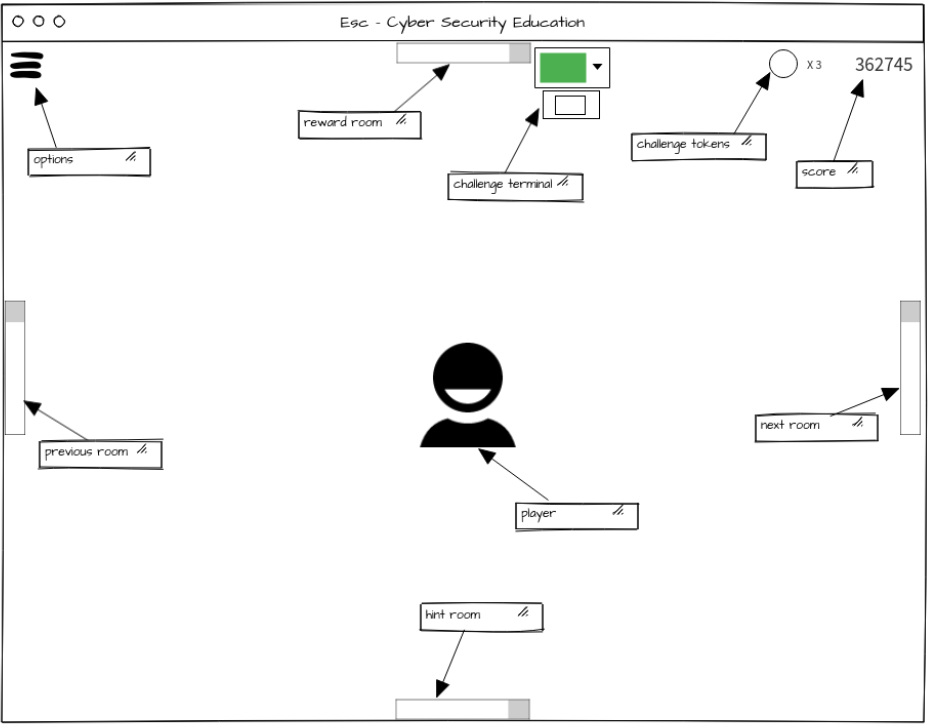
\includegraphics[width=1.0\textwidth]{Figs/Ui_main_screen.PNG} 
    \caption{Main Screen UI mock up} 
    \label{Mainscreen}
\end{figure}   

The main screen has quite a lot going on. In a typical room, the player will have a choice to navigate both to the next room and the previous room to their left and right. If they go up they will reach the challenge terminal which when interacted with brings up the challenge. If they enter the correct answer the reward room will open up and they can collect their challenge token. If they get it incorrect the hint room below opens up. How many Challenge tokens they have is displayed and also the score they have accumulated so far. The user can quit or alter their settings with the drop down menu in the top left hand corner of the screen. (Figure \ref{Mainmenu}) (Figure \ref{fig:test1}) (Figure \ref{fig:test2})

\begin{figure}[h]
    \centering
    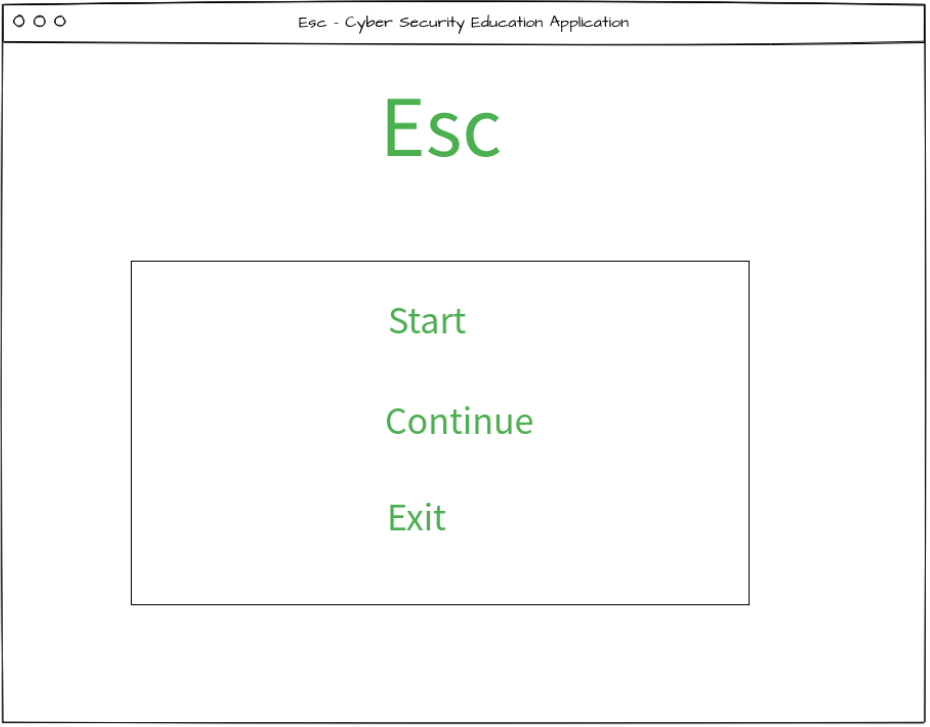
\includegraphics[width=1.0\textwidth]{Figs/Ui_main_menu.PNG} 
    \caption{Main Menu UI mock up} 
    \label{Mainmenu}
\end{figure}   

\begin{figure}
\centering
\begin{minipage}{.5\textwidth}
  \centering
  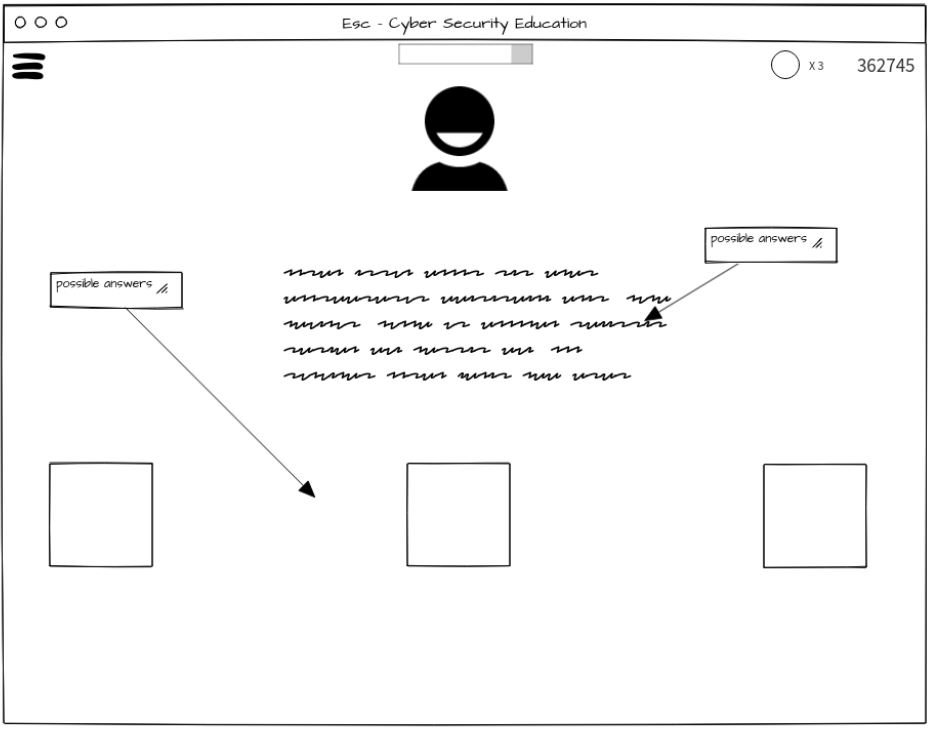
\includegraphics[width=1\linewidth]{Figs/Ui_hint_room.PNG}
  \captionof{figure}{Hint room}
  \label{fig:test1}
\end{minipage}%
\begin{minipage}{.5\textwidth}
  \centering
  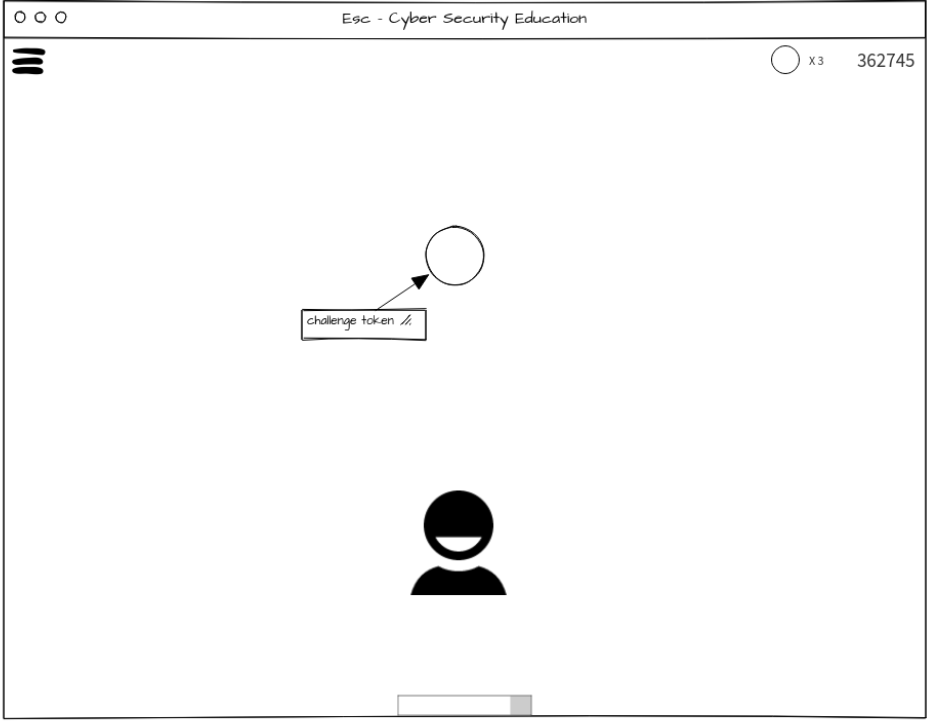
\includegraphics[width=1\linewidth]{Figs/Ui_reward_room.PNG}
  \captionof{figure}{Reward room}
  \label{fig:test2}
\end{minipage}
\end{figure}   

When the user enters the hint room they are presented with a question and a choice of three answers. They will get the hint regardless but is meant to build their knowledge and whats been covered. The reward room is simple and just contains the challenge token. (Figure \ref{fig:test3}) (Figure \ref{fig:test4})

\begin{figure}
\centering
\begin{minipage}{.5\textwidth}
  \centering
  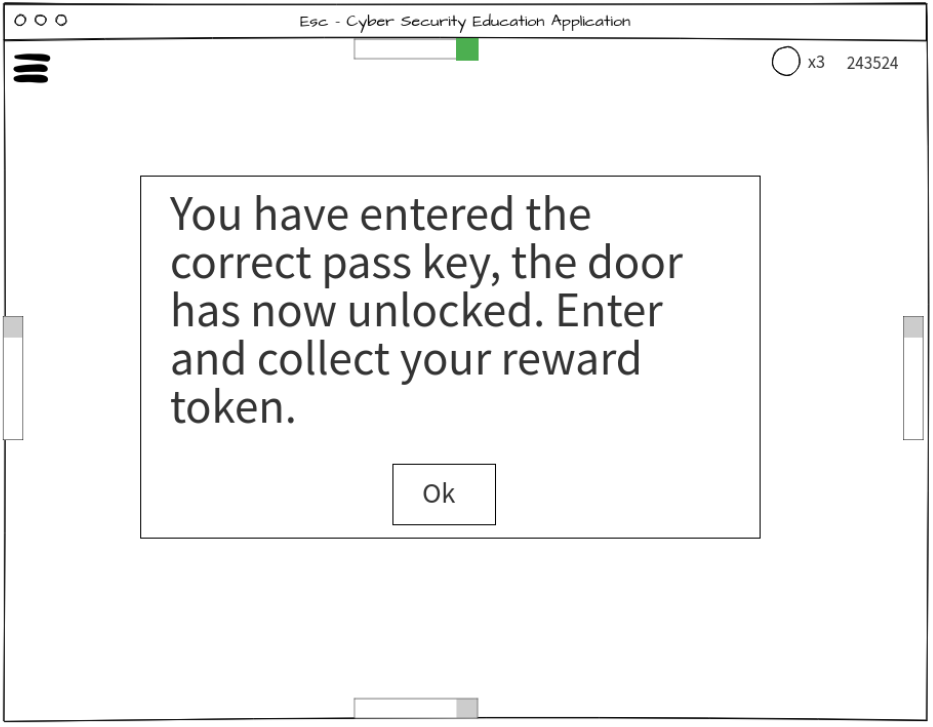
\includegraphics[width=1\linewidth]{Figs/Ui_correct_response.PNG}
  \captionof{figure}{correct response screen}
  \label{fig:test3}
\end{minipage}%
\begin{minipage}{.5\textwidth}
  \centering
  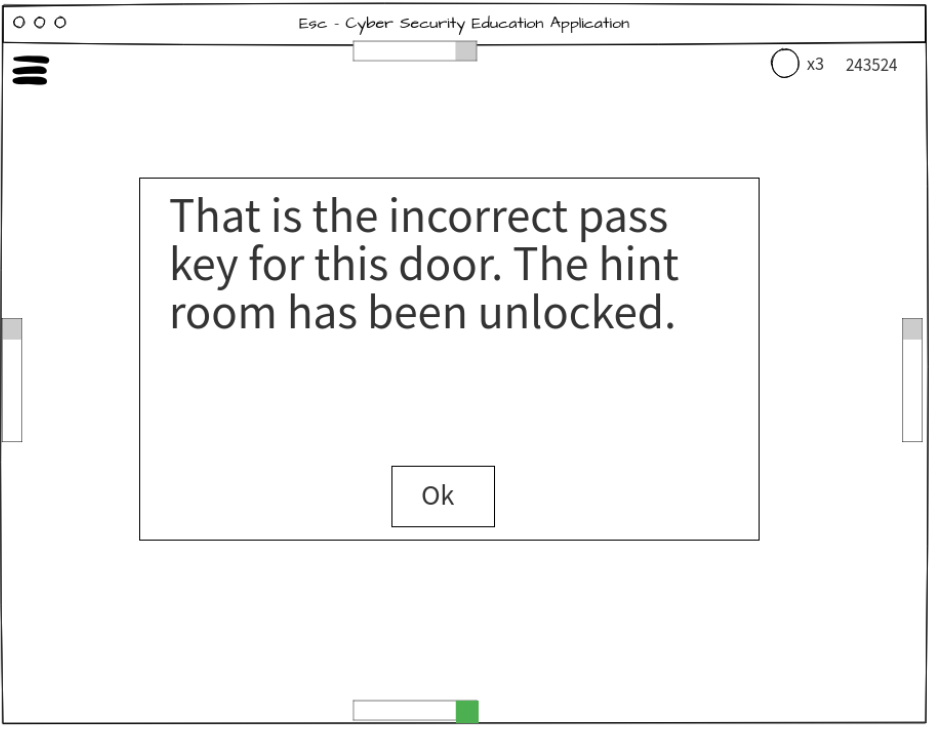
\includegraphics[width=1\linewidth]{Figs/Ui_incorrect_response.PNG}
  \captionof{figure}{incorrect response screen}
  \label{fig:test4}
\end{minipage}
\end{figure}  

The feedback received at this level is basic but dependent on what the answer is different doors unlock.

%insert annotated mockflow screens%
{Register/Home screen} 
{Room screen} 
{Reward screen} 
{Hint screen}
\subsection{Middle end}  
\subsubsection{Challenge Generator}  
One fundamental part of this application will be the challenge generator. Dynamic challenge generation is an important element of this application, it will ensure that if the user comes back and does it again they will have a different experience and also that users will be having a different experience than the users around them. I will look at three possible methods of dynamic challenge generation. \emph{Random challenge selection, API request} and \emph{Web scraping}.  

\emph{Random Challenge selection} 

This will involve setting up a list of possible questions with corresponding answers, then selecting one of those questions at random. I will ask a multiple choice question populated with the correct answer and the answers to the other questions. The script would them check for the user input and check if the answer matches the correct answer giving simple feedback accordingly. This will be the simplest method and the easiest to implement (Figure \ref{RandomSelection}).  

\begin{figure}[h]
    \centering
    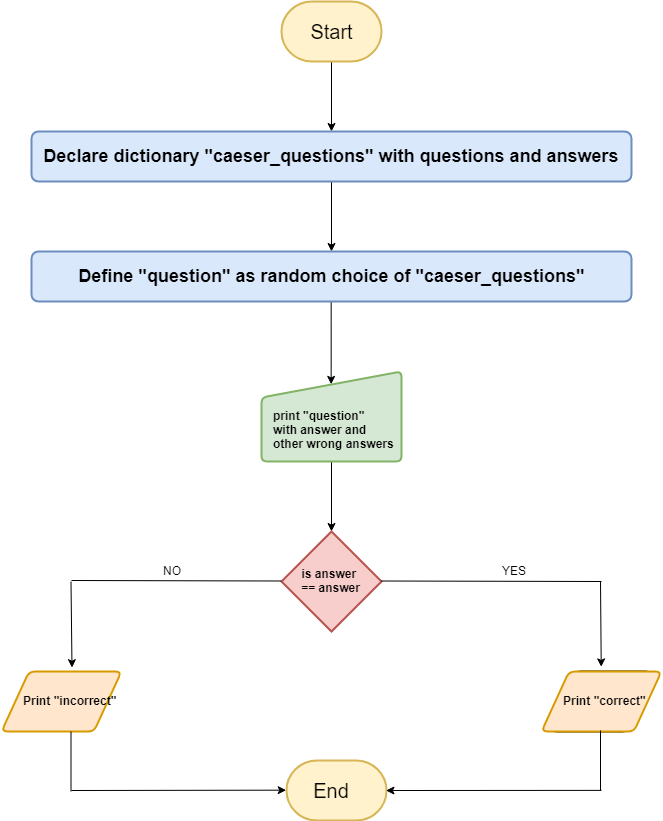
\includegraphics[width=0.5\textwidth]{Figs/random_selection (1).png}
    \caption{random selection flow chart} 
    \label{RandomSelection}
\end{figure}   


\emph{API request} 
I will set up an API using a python script so I can make a request to it with another script. The script will select a random word from a list, the world will correspond with a question that the API will send back when it receives this word. The user will then send back the answer which will be sent to the API and checked (Figure \ref{APIRequest}).   

\begin{figure}[h]
    \centering
    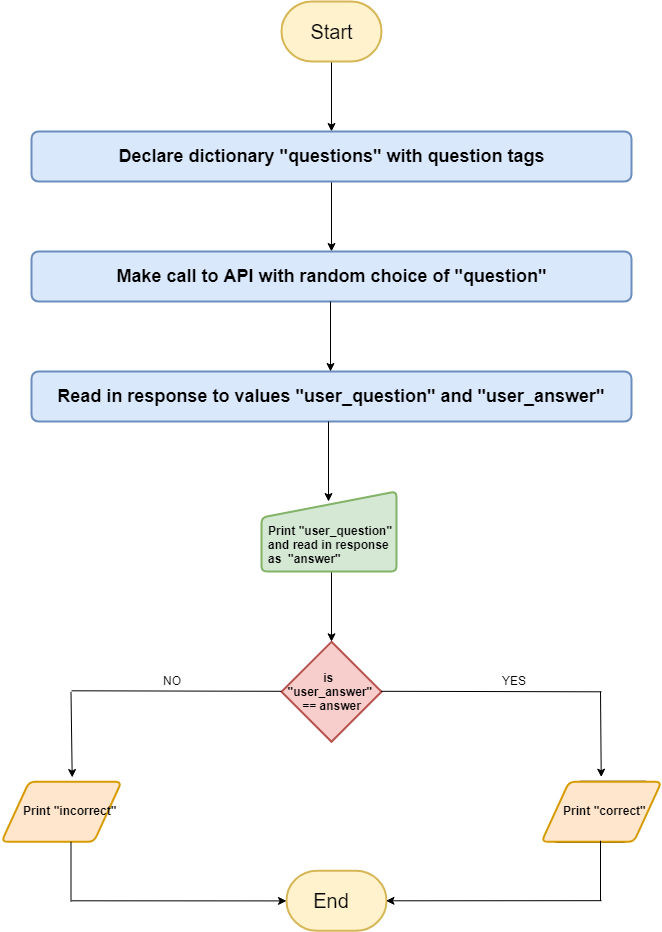
\includegraphics[width=0.5\textwidth]{Figs/API_request.png} 
    \caption{API request flow chart} 
    \label{APIRequest}
\end{figure}   


\emph{Web Scarping} 
I will develop two web scraping applications to test the effectiveness of it as a method of dynamic challenge generation, one simpler one and one more complex. for the more simple one I will scrape the names of influential computer scientists from sites like either 'https://www.computerscie
ncedegreehub.com/30-most-influential-computer-scientists-alive-today/' this or a Wikipedia entry on something similar. Then will read those names into a list. The challenge would be generated by grabbing a random name from that list and running it through an online hash generator, providing all the information you need for the challenge (Figure \ref{WebScraper}).   

\begin{figure}[h]
    \centering
    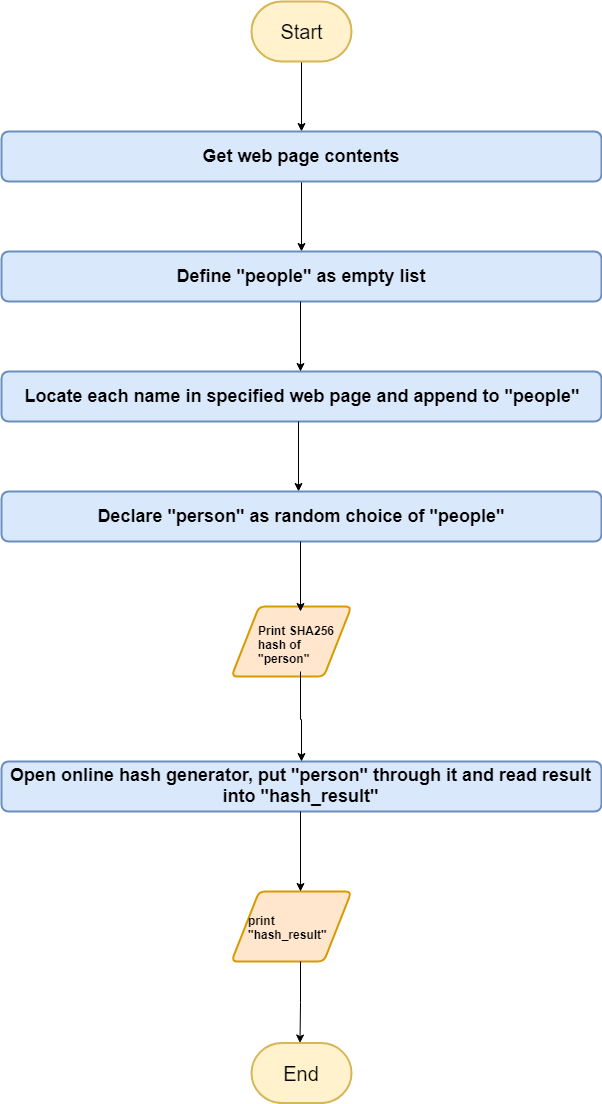
\includegraphics[width=0.5\textwidth]{Figs/Web_scraper.png} 
    \caption{Web scraper flow chart} 
    \label{WebScraper}
\end{figure}   


The more complex use of web scraping would involve using the Bing API and the Microsoft cognitive engine. The script would ask the Bing API for 100 cryptographers, it would then store images of them in a list, returns one at random and sends it to the Microsoft cognitive engine to see if it recognised it. This script would be used to ask the users if they recognise the famous cryptographers and check their answer against the answer returned from the Microsoft cognitive engine. (Figure \ref{FaceQuiz})   

\begin{figure}[h]
    \centering
    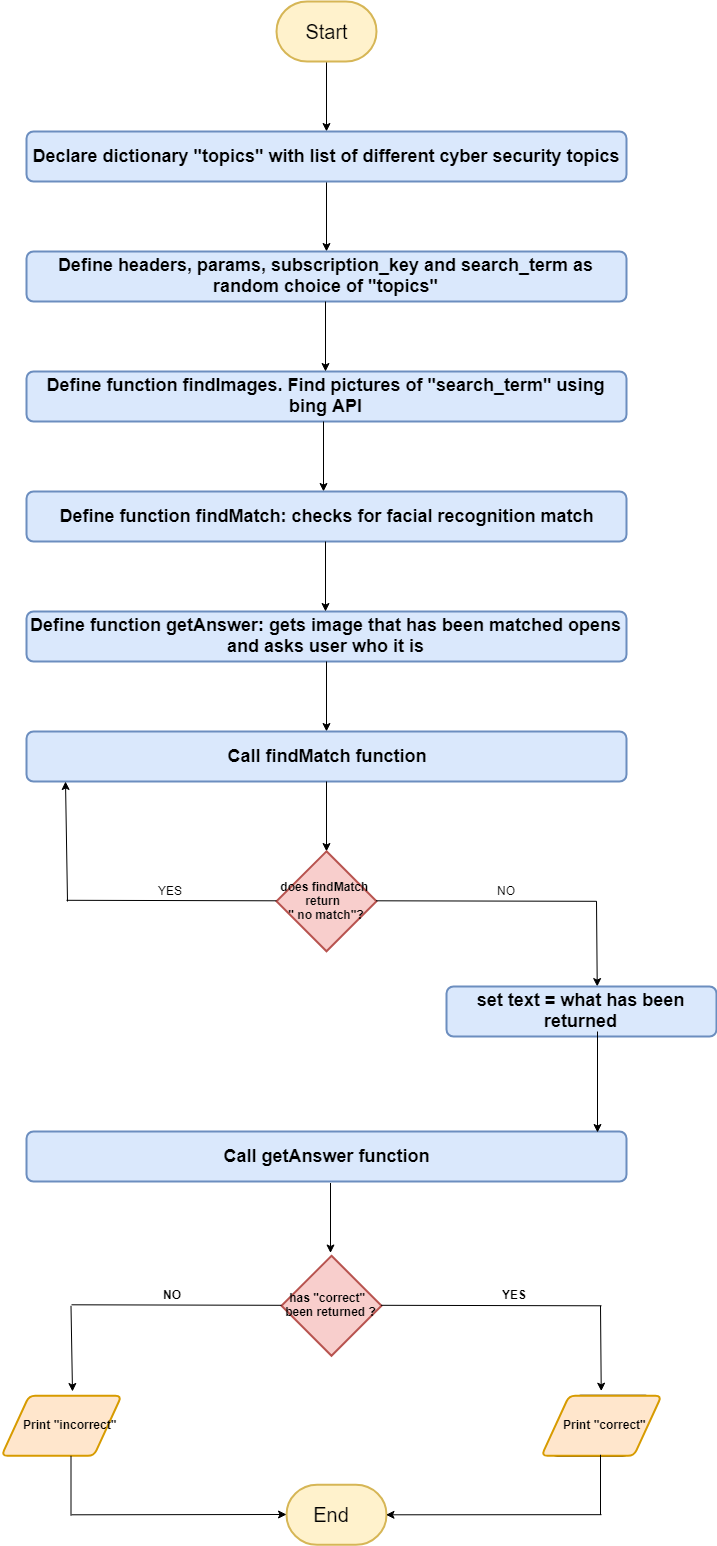
\includegraphics[width=0.5\textwidth]{Figs/Face_Quiz (1).png}
    \caption{Face Quiz flow chart} 
    \label{FaceQuiz}
\end{figure}    

\emph{Docker} 
%talk about use of docker  
(Figure \ref{DockerFace})

\begin{figure}[h]
    \centering
    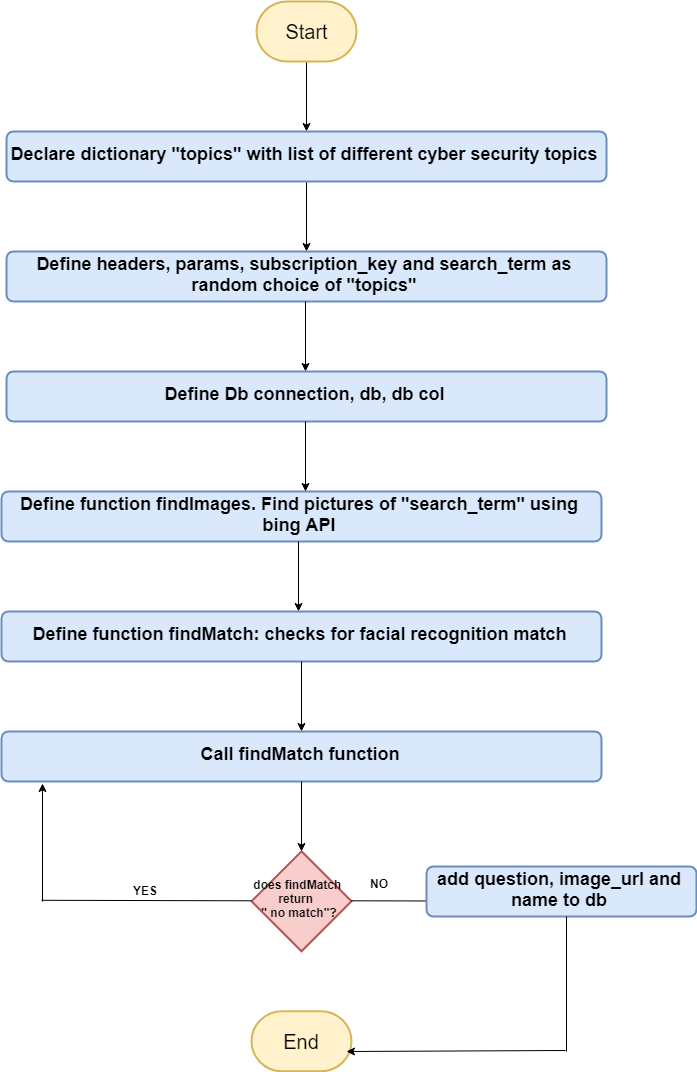
\includegraphics[width=0.5\textwidth]{Figs/Docker_face_pop.png} 
    \caption{Docker face pop flow chart} 
    \label{DockerFace}
\end{figure}   




%literature to back up dynamic challenege generation%
\subsubsection{Feedback} 
As discussed in the literature, Feedback is fundamental to an educational application.  
\subsection{Back end} 
\subsubsection{SQL vs NoSQL}   
First off when designing the back end of an application what Database would be most efficient to use for the applications specific needs and potential uses. 
%reference and and back up use of NOSQL and mongo DB (also discuss that managing the database part of the application when it comes to scaling because a lot of the load comes from complex queries making requests take longer, so techniques such as cacheing complex query results and effective organising of db tables with keys and index can be effective in reducing load. %
\subsubsection{User Database}   
Discuss the user database (Figure \ref{UserDB})

\begin{figure}[h]
    \centering
    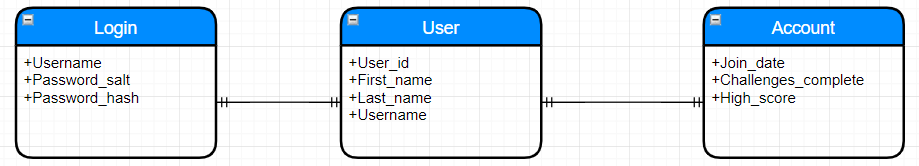
\includegraphics[width=1.0\textwidth]{Figs/User_Db.PNG} 
    \caption{User Database} 
    \label{UserDB}
\end{figure}   

\subsubsection{Challenges Database}   
Discuss The challenge Database (Figure \ref{ChallengeDB})

\begin{figure}[h]
    \centering
    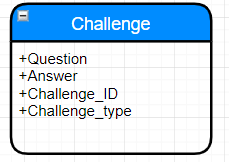
\includegraphics[width=0.5\textwidth]{Figs/Challenge_Db.PNG} 
    \caption{Challenge Database} 
    \label{ChallengeDB}
\end{figure} 

\subsubsection{Results Database}   
Discuss the results database (Figure \ref{ResultsDB})

\begin{figure}[h]
    \centering
    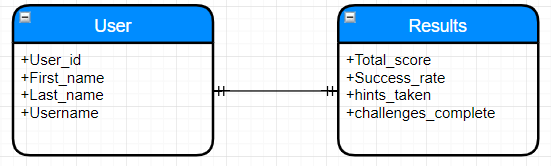
\includegraphics[width=1.0\textwidth]{Figs/Result_Db.PNG} 
    \caption{Result Database} 
    \label{ResultsDB}
\end{figure} 

\subsubsection{Back end Framework} 
With angular being chosen as the front end framework a similar evaluation needs to be done when choosing a back end framework that can work in conjunction with it.
\subsection{Other utelized services} 
\subsubsection{Github}  
Github is an online code repository which can be used to keep track of software development updates and allow your code to be open source. 
%more on githb ad how I could use in cpnjunction with docker% 
\subsubsection{Docker}  
Docker is a way of taking an forxen state of an application or "image" and running it as multiple "containers" which are similar to virtual machine instances except  
%insert difference here and more about docker and how it could be used for my application% 
\subsubsection{Load Balancing} 
Load balancing is a way of handling a server traffic so that multiple requests get distributed between multiple servers, therefore reducing the load on each server and has been researched and used as way of scaling web applications \cite{chieu2009dynamic}.

%bit of research on load balancing e.g different algorithms such as random, round robin, and load based. 

\section{Implementation}
After the research had been done and I had designed in theory what my application would look like and how it would work I could start to look at the implementation. I decided for my implementation to prototype certain parts of my theoretical design. I chose to prototype the dynamic challenge generation part of the project as I felt that it was an important part of the learning experience to make sure that a different challenge could be given to a user each time they used the application, or if it was used in a class to ensure that all the users had different experience's using the application and couldn't copy other users answers out of laziness. Dynamic challenge generation was also an interesting area to look at I thought it would be interesting to evaluate the effectiveness of the different approaches in creating a different challenge each time. Another part I decided to prototype was the docker element of the project as docker is an incredibly useful service which would benefit the project greatly if made and prototyping an element such as database population would help illustrate that as well as gauge how efficient it would be.  

For the implementation stage I decided to use Python for the programming language and Eclipse as the IDE. I chose python out of a mix of personal preference as I has used in in the years leading up to this project and had more experience than any of the other programming languages and the practicality of using it for this project as python has extensive support libraries, useful for completing the variety of tasks that I wanted to do, combined with the fact that it is a widely used language and recognised in the industry it seemed like a sensible choice. Eclipse I chose to use as I have has exposure with it in my uni career and thought it better to use something I am experiences with and know than learn the specifics of a new IDE.

I will use the Eclipse IDE to develop python scripts for the different methods of dynamic challenge generation, at least a script for each. I will then use a combination of docker and python to create a service which populates a database with challenges in an efficient matter. The aim of this implementation stage is to develop something that in a later stage will give an understanding into which method of dynamic challenge generation is the most effective and how to best distribute this method.   

%include code snippets here, explain what they do etc. all scripts and docker files

%need to talk about testing strategy, how am I going to test it ? 
\subsection{From selection} 
\subsection{Using API request} 
\subsection{Web scraping} 
\subsubsection{Basic web scraping} 
\subsubsection{Web scraping with facial recognition} 
\subsection{Challenge distribution with Docker} 
\subsubsection{Python} 
\subsubsection{Docker} 

\section{Results} 
%Results for for tests:out of X runs how many times did the same question show up ? to evaluate the three dynamic challenge generation method. test how many faces show up in search out of 100 ? to evaluate bing API effectiveness for different topics such as computer scientists and cryptographers. Out of 100 faces how many correct ? to evaluate facial recognition. Then evaluate further effectiveness of facial recognition by taking 100 famous computer scientists, cryptographers etc of varying fame level, very famous to kind of famous to not very famous and test success rate. feed it some duds, Bill Gates look a like etc. 

\section{Evaluation}
Evaluate my literature and implementation as a whole. 

\section{conclusion} 
\subsection{Aims and Objectives} 
\subsection{Self Evaluation} 
\subsection{Future Work}

\newpage
\bibliographystyle{IEEEtran}
\bibliography{Diss_papers}
%example of References. See https://en.wikibooks.org/wiki/LaTeX/Bibliography_Management
%might be good to use a separate document for these so your main work is not one really long text file. 

%you can crate this on a extra tex document just like the title or any other part of the document.
\newpage
\begin{appendices}
\section{Project Overview}
%insert IPO

\begin{subappendices}
\subsection{Example sub appendices}
...
\end{subappendices}

\section{Second Formal Review Output}
Insert a copy of the project review form you were given at the end of the review by the second marker

\section{Diary Sheets (or other project management evidence)}
Insert diary sheets here together with any project management plan you have

\section{Appendix 4 and following}
insert content here and for each of the other appendices, the title may be just on a page by itself, the pages of the appendices are not numbered, unless an included document such as a user manual or design document is itself pager numbered.
\end{appendices}

\end{document}
